\documentclass{article}
\usepackage{graphicx}
\usepackage{epsfig}
%\usepackage{pdflatex}
\title {SuperBigBite Data Acquisition Implementation}
\author{Alexandre Camsonne}

\begin{document}
\section{Introduction}
\subsection{CODA}
Jefferson Laboratory is using the Cebaf Online Data Acquisition system for data taking.
CODA is based on a main server interacting with a database in which all the DAQ components update their status . The readout crates host a single board computer running a Read Out Controller (ROC) program which controls and reads out the data from the electronics. The ROCs send the data through a standard network link usually ethernet to a computer running the Event Builder program, which uses the data from the ROC to check synchronization and build the event. Finally the event is sent to the Event Recorder which puts the event into a file on the hard drive of the computer.
In addition to the software a set of harware components specific to CODA is used in order to keep ensure event synchronization between all the components each crate has a trigger interface ( TI board ) which sends the trigger signal to the ROC program for the read out of the data. All the TI are linked to a trigger supervisor board which takes the triggers and sends them to the TI while monitoring the status of each TI to keep all the crates synchronized and generates a Level 1 accept and Level 2 accept for the read out modules. The TS also takes as input the front end busy of the modules to inhibit the triggering if one module is not ready insuring synchronization between the modules.


\subsection{SuperBigBite}
The SuperBigBite spectrometer will be use for several experiments in different configuration. The main elements are a large dipole magnet associated with large GEM trackers to provide the postion of the particles allowing to determine their momentum.
\section{Detectors}
In addtion to the SuperBigBite spectrometer several additionnal detectors will be used.
\subsection{Electron electromagnetic}
The Electromagnetic Calorimeter will have 1920 lead glass blocks arranged in a matrix 60x32 ?. The electromagnetic calorimeter trigger is done by analog summing. 
The front-end system includes 122 custom NIM 2x8 amplifier/summers, 60
4x4 NIM summers, 8 16 chan. NIM discriminators, 9 16 chan. NIM logical OR.
Total of 20 NIM crates for the front-end electronics. Total 2050 RG58 500 ns
cables from the front-end to the DAQ. They would be connected to the 64
BNC-34 patch panels (32 on the front-end side and the same number on the
DAQ side). 
The DAQ system includes 12 FastBus crates with 4 power supply units, 12 SFI
modules, 12 CPUs and 12 TI’s, 96 ADCs 1881m and 6 TDCs 1877S.

\subsection{Hadron calorimeter}
This hadronic calorimeter will be used as proton and neutron trigger.
It has 24x12 = 288 channels. The readout and trigger will be done using FADCs.
For the neutron experiment the detector will also give the neutron momentum by measuring the time of flight. In this configuration we plan to split the signal between FADC and discriminator to go to high resolution TDC.

\subsection{Coordinate detector}
The coordinate detector is an array of 2352 thin planes of scintillators readout by multianode PMTs. They will have a front end electronics based on the NINO chips which will give a discriminated signal for all the channels. The logic signals will be fed to Fastbus TDC 1877S. 
\subsection{Big Bite Spectrometer}
The Big Bite spectrometer is part of standard Hall A equipment it is a smaller dipole with a detector stack.
\subsubsection{Electromagnetic calorimeter}
The main electron trigger is the shower detector. The shower is 7x27 lead glass blocks. An analog sum of 7 blocks is made. This sums are further added using 4 channels linear fan module.
A preshower layer 2x27 is placed in front of the shower but is usually used off line for pion electron identification. This make a total of 189 + 54 = 243 lead glass blocks to be readout.
The readout of the detector will be done using fastbus.
\subsubsection{Scintillator array}


\subsubsection{Gas Cerenkov detector GRINCH}
\subsubsection{GEM }

\subsection{Detector configuration summary}
\begin{tabular}{|c|c|c|c|c|}
\hline
Experiment&Trigger rate & Detectors & Subdetectors & Channels\\
\hline
GEp5& 3 KHz  & SBS & Front tracker & 60,000\\ 
 && & Back tracker & 64,000\\
 && & HCAL & 288\\
 & & Electron arm& ECAL & 1920 \\ 
 &&              & CDET & 2352 \\ 
\hline
GEn& & SBS & HCAL & 288 \\ 
 &    &   & CDet & 2352 \\ 
 && BigBite& Shower & 243\\ 
 && BigBite& Scintillator & 243\\ 
 && BigBite& Gas Cerenkov & 243\\ 
\hline
GMn& & SBS & HCAL & 288 \\ 
   &  &   & CDet & 2352 \\ 
 && BigBite& Shower & 243\\ 
 && BigBite& Scintillator & 180\\ 
 && BigBite& Gas Cerenkov & 243\\ 
 && BigBite& Front tracker & 60000\\ 
 && BigBite& Back tracker & 640000\\ 
\hline
Transversity && SBS & Front tracker & \\
 &&  & Back tracker & \\
 &&  & RICH & \\
 && Big Bite & Front tracker & \\
 &&  & Back tracker & \\

\end{tabular}


\section{GEM readout}
The GEM readout is carried out by the APV25 chip. It a pipelined ASICs with 128 channels and pipeline depth of 192 samples sampling at 40 MHz. When a trigger is issued the corresponding cells are frozen until they are readout while the other cells are still being used reducing the dead time.
For each trigger all the data of 128 channels are transfered at 40 MHz rate in a multiplexed analog format. Adding some header and event informations 141 words are transmitted for each trigger which gives a transfer time of $141x25 ns = 3.6 \mu s $. In case of high background several consecutives time samples can be sent in order to detect pile up, we plan to read 3 samples which gives a transfer time of 10.8 $\mu s$. This allows deadtimeless operation for rates up to 90 KHz. The readout planned to be use the the INFN Multi Purpose Digitizer (MPD), it is a VME board with a 200 MHz FADC and signals to control the APV setup and readout. 


\section{Pipelined electronics, HCAL trigger}
The hadron calorimeter will be read out by the JLAB pipelined electronics.
The central module for this system is the JLAB FADC250, a 16-channel 12-bit FADC sampling at 250~MHz. The input signals are continuously recorded into the memory with a memory depth up to 8 us. The system is thus dead timeless as long as the trigger is generated before the memory rolls over and the event of interest is overwritten.
The Flash ADC has two separated data path.
The first one uses the new high speed serialized VME standard called VME switched Serial (VXS).
It allows full duplex point to point connection at up to 2.5 Gbps per lane using the backplane central connector.
Currently the FADC is using two VXS lanes giving 5 Gbps of bandwidth.
This allows to transfer a 16 bit word from each FADC to a Crate Trigger Processor (CTP) board every 4~ns.
Each FADC being connected to The CTP via a 5 Gbps link, the CTP uses up to 16 FADC words from each FADC to form a 32-bit word every 4~ns which can be a lower resolution sum of all the channels or a bit pattern of the channel hit for example.
The CTP board then sends the processed signals to a Sub-System Processor (SSP) board via a 10 Gbps optical link which puts together all the data from individual crates and computes the associated quantities which will be used in the trigger.
All the SSP boards send their processed information to a Global Trigger Processor (GTP) which makes the L1 trigger.
The GTP sends the trigger to the Trigger Supervisor (TS) which makes sure the system is ready to accept a trigger and sends the accepted signal to the Trigger Distribution boards in the VXS crates which are linked to the Trigger Interface boards in each crates via optical link as represented in Fig.\ref{fig:pipeline_daq}.
The trigger and synchronization clock signals will then be sent back to individual crates and payload modules through Trigger Interface/Distribution (TID) boards and Signal Distribution (SD) boards which distributes the signals to the electronics such as the FADC.
Once a trigger is generated, the full resolution data which is still in the pipeline is readout out using the VME320 protocol at an average data rate of 200 MB/s.
The Flash ADC can run in different modes, it can either transfer all the samples of the waveform which can be useful to study pileup effect and background or process the data to give an integral over the length of the pulse.

\begin{figure}
  \centering
  % Requires \usepackage{graphicx}
\includegraphics[width=\textwidth]{figs/TriggerPipeline.pdf}\\
  \caption{Standard Triggering scheme using the JLAB pipeline electronics}\label{fig:pipeline_daq}
\end{figure}

The CTP having all the amplitude of all the calorimeter, it can compute all the sums of adjacent blocks.
A sum of 3$\times$3 blocks was implemented.
In order to reduce the number of triggers coming from the background this summing approach is chosen to improve the online pion rejection.
A sum over 1 central block and 6 surrounding blocks can be implemented in the same way as the HPS scheme.

\begin{figure}
  \centering
  % Requires \usepackage{graphicx}
 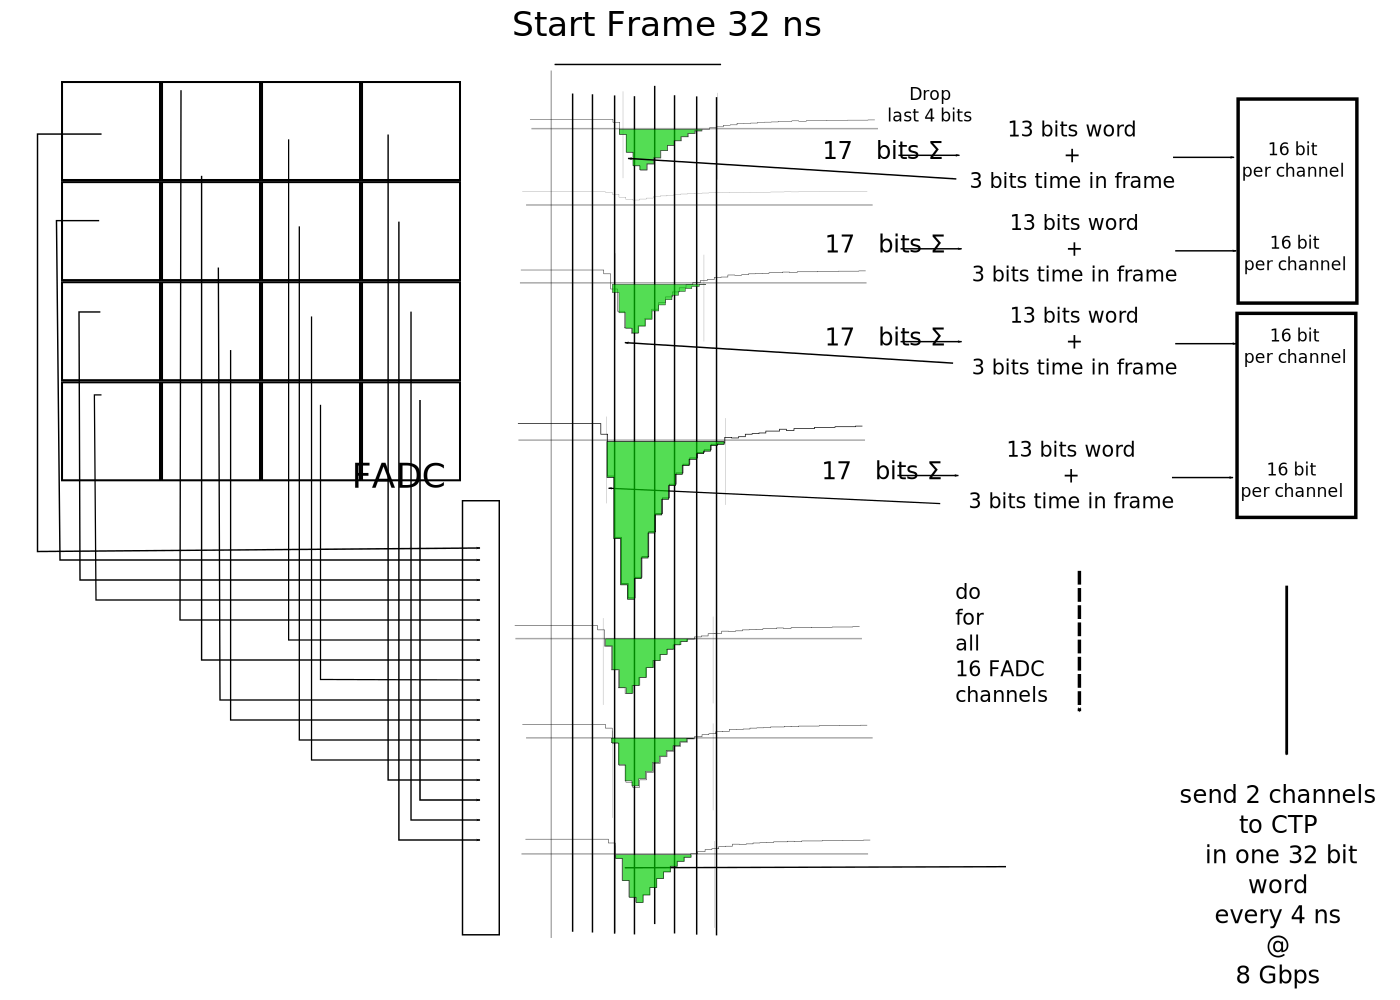
\includegraphics[width=\textwidth]{figs/CaloTrigger.pdf}
  \caption{Calorimeter clustering scheme using the HPS algorithm. All calorimeter signals are sent to the FADC. }\label{fig:ClustHPS}
\end{figure}

\begin{figure}
  \centering
  % Requires \usepackage{graphicx}
  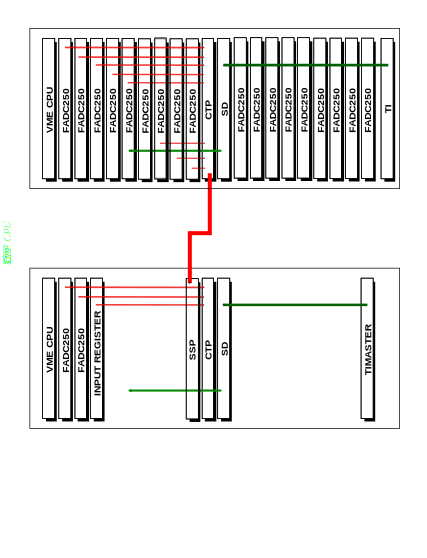
\includegraphics[width=\textwidth]{daq/figs/VXSHCalFADC.pdf}\\
  \caption{HCAL crate layout }\label{fig:HCALFADC}
\end{figure}

\section{Fastbus}
Fastbus is an electronics standard . It can transfer up to 10 Megawords per second with a 32 bit width which gives a maximum theoretical throughput of 20 MB/s.
Since we have a lot of Fastbus equipment on hand. It will be used in order to save money for the large number of detectors channels. The main readout is the Lecroy ADC 1881M a 13 bit ADC, with a 9 $\mu$s encoding time in 12 bit resolution and 12  $\mu$s. The 1881M features a fast clear and is ready to tahe another event after 1 $\mu
The Struck Fastbus Interface is a Fastbus Master which translates 

\begin{tabular}
\hline
\end{tabular}


The Form Factor experiment Gep5

\begin{tabular}{|c|c|c|c|}
\hline
Experiment & GEM channels & additional detectors & Trigger rate\\
Gep5 & &Electromagnetic calorimeter& 3 KHz \\
GEn& & &Hadron calorimeter\\
GMn&& Hadron calorimeter\\
Transversity&&Hadron calorimeter\\
\hline
\hline
\end{tabular}

\section{Data acquisition for GEp5 experiment}
\subsection{Requirements}
\subsection{Detectors}
\subsection{Trigger}
\subsection{Event size and data rates}
\section{Data acquisition for GEn experiment}

\section{Data acquisition for GMn experiment}


\section{Data acquisition for transversity experiment}

\section{A1n}

\section{Inventory}

\section{Manpower}

\section{Timeline and milestones}

\section{Budget}
\end{document}
